\section{Vågutbredning på kortvåg}
\textbf{
HAREC a.\ref{HAREC.a.7.7}\label{myHAREC.a.7.7}
}
\index{vågutbredning!kortvåg}
\index{vågutbredning}

\subsection{Markvåg}
\index{markvåg}
\index{vågutbredning!markvåg}

\emph{Markvågen} (eng. \emph{ground wave}) breder ut sig längs jordytan utan
kontakt med atmosfären genom reflexion eller refraktion.

Markvågen har vertikal polarisering och en vertikal vågfront när
jordplanets ledningsförmåga är god.
Vid sämre ledningsförmåga lutar vågfronten framåt.

Markvågens räckvidd står i förhållande till den använda frekvensen,
sändareffekten och jordplanets ledningsförmåga.

Vid frekvenser under ca 10~MHz är jordytan är en tämligen god ledare.
Markvågsutbredning utnyttjas därför mest vid låga frekvenser, till exempel för
rundradio i lång- och mellanvågsbanden då räckvidden kan vara i
storleksordningen 1000~km.
På kortvåg är markvågsräckvidden i 80~meters-bandet ca 100~km och i
10~meters-bandet ca 15~km.

\subsection{Rymdvåg}
\index{rymdvåg}
\index{vågutbredning!rymdvåd}

Under vissa förutsättningar reflekteras radiovågorna mot joniserade
atmosfärsskikt och når åter jordytan på stort avstånd från utsändningspunkten,
då kan man använda \emph{rymdvåg} (eng. \emph{space wave}).
Rymdvågsutbredning utnyttjas mellan platser på jordytan med stort avstånd.

För att bäst uppnå den önskade reflexionen måste man dels välja
lämplig tidpunkt och frekvens och dels utforma antennen så att den har
sin huvudriktning i en bestämd vinkel mot det reflekterande skiktet.

Jonosfären är den del av atmosfären på ca 50 till 350~km höjd, där
instrålningen från solen skapar fria elektroner och joner i en sådan
mängd att det bildas skikt med god elektrisk ledningsförmåga.
Under vissa villkor reflekterar dessa skikt radiovågorna, men kan under
andra villkor även absorbera dem.

\begin{figure}
  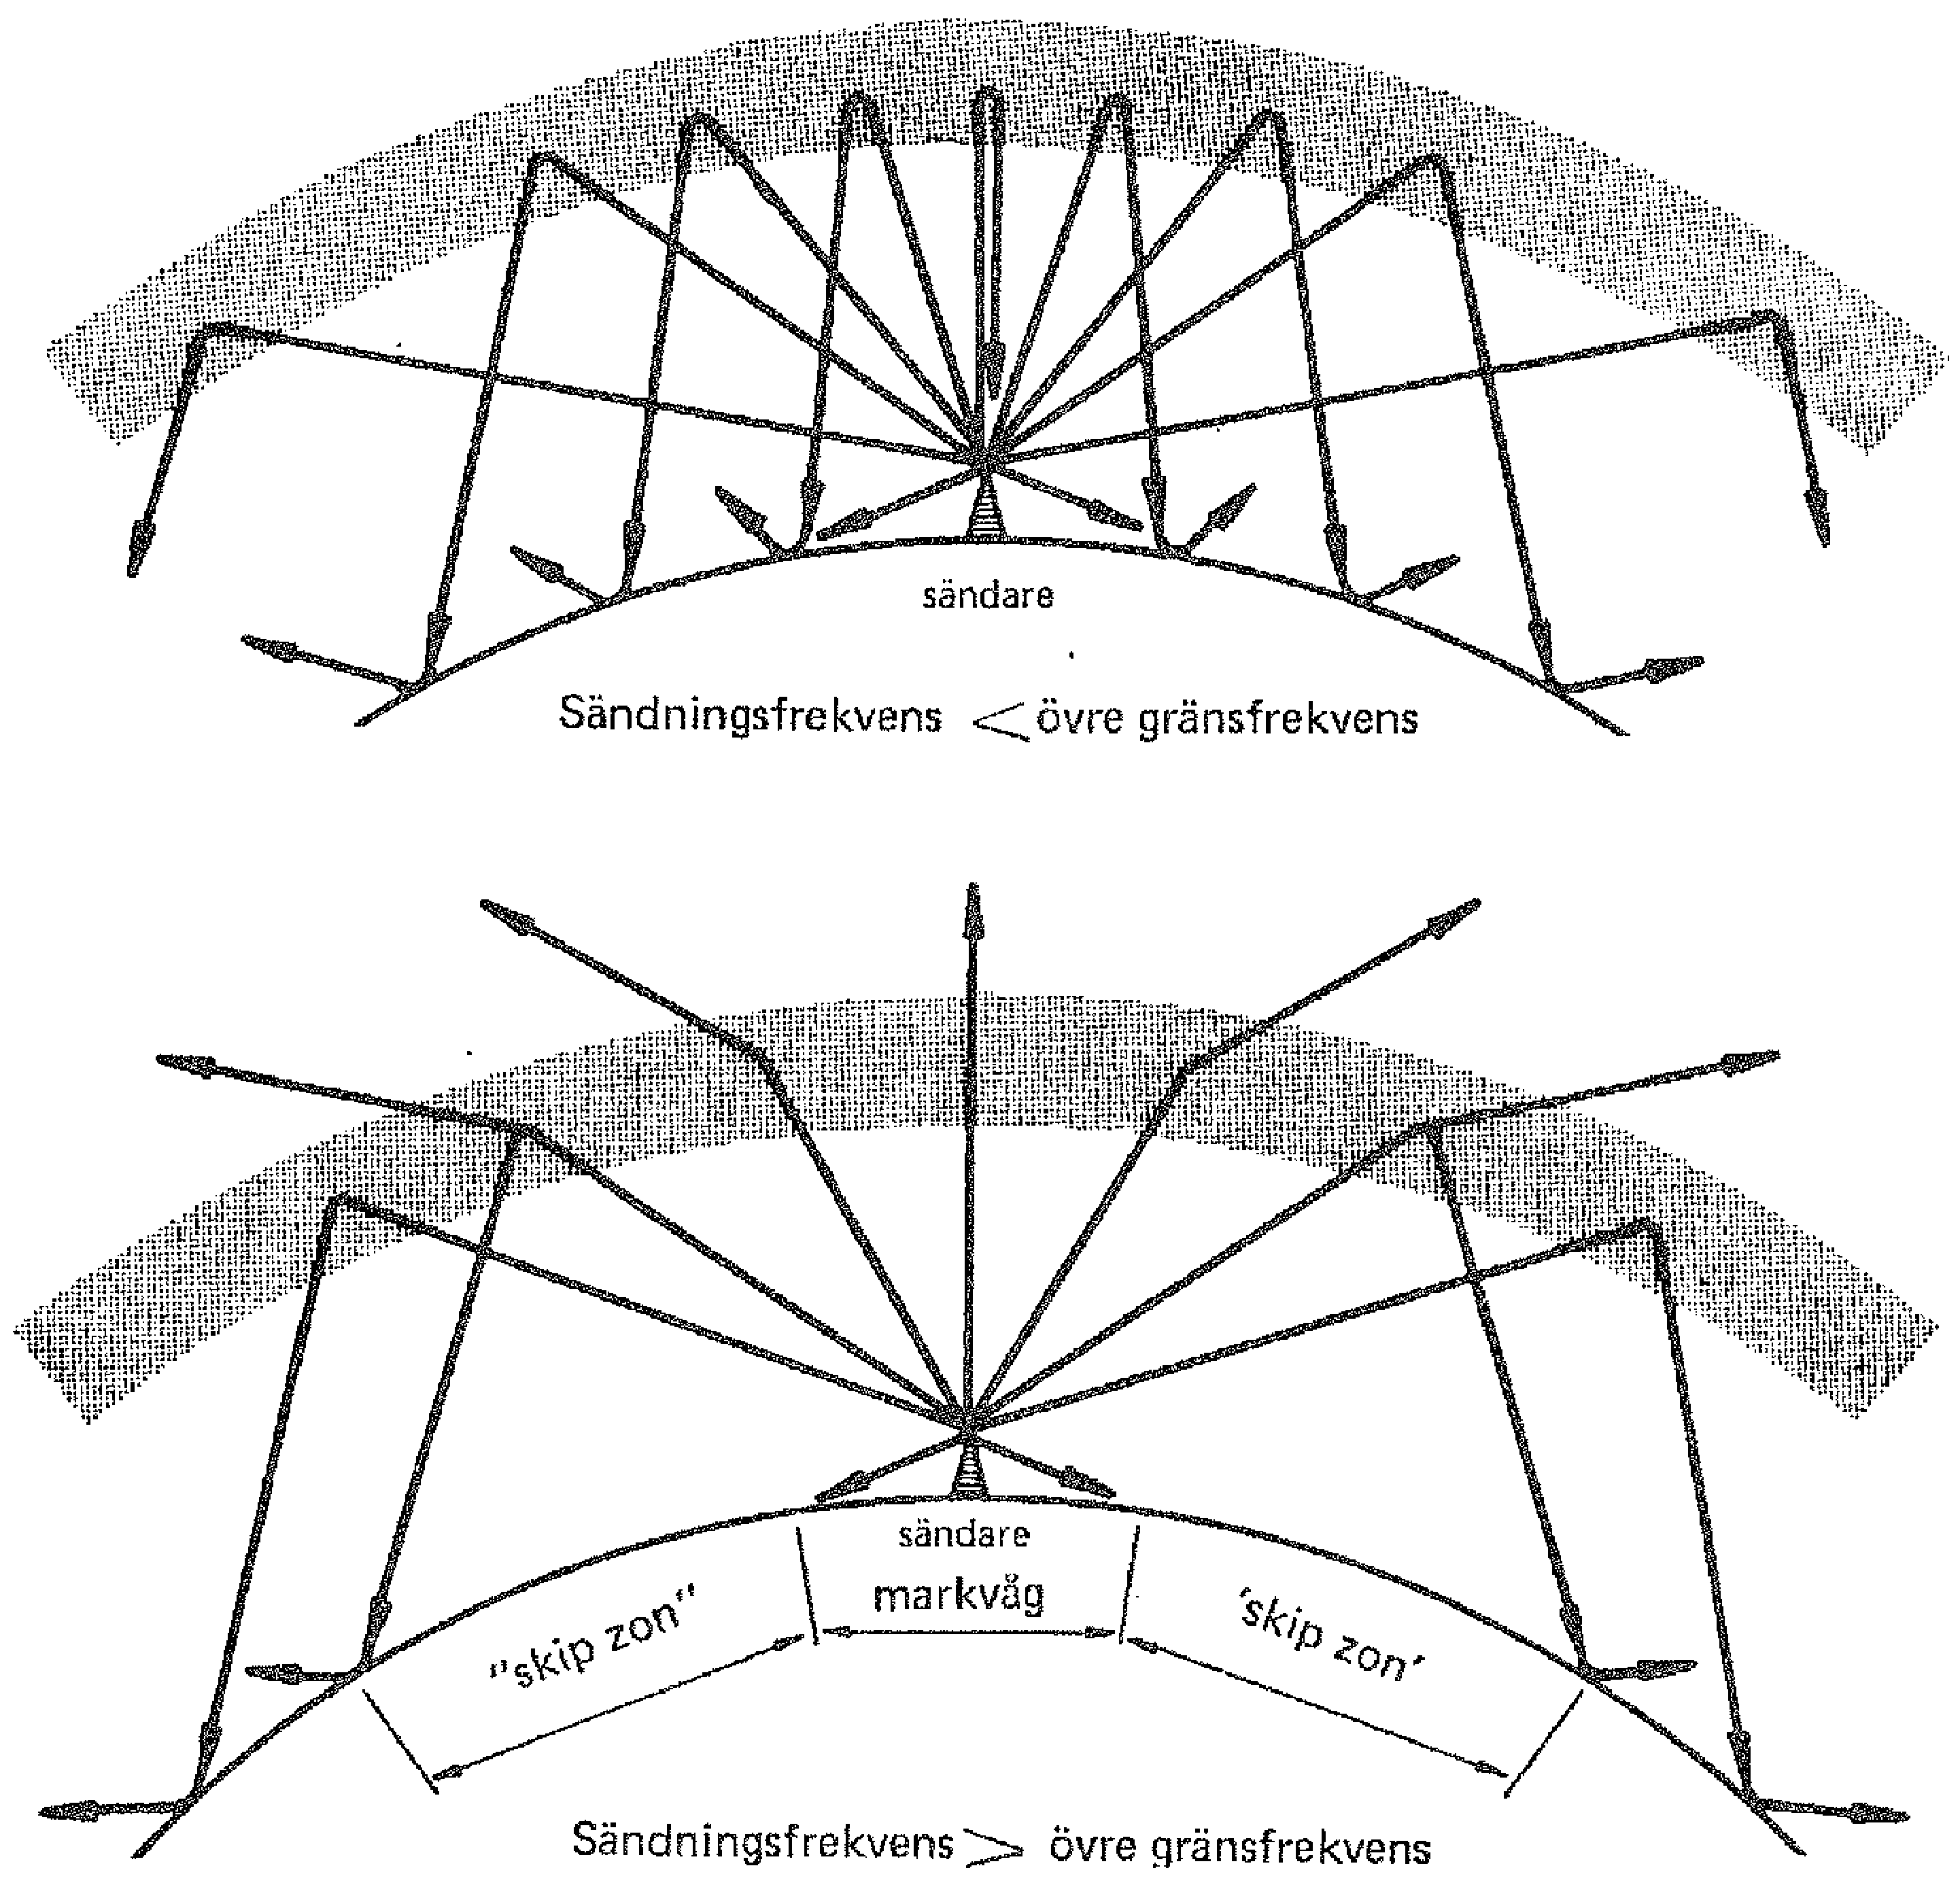
\includegraphics[width=\textwidth]{images/cropped_pdfs/bild_2_7-11.pdf}
  \caption{Vågutbredning på kortvåg}
  \label{fig:bildII7-11}
\end{figure}

När vågorna från jordytan reflekterats mot de joniserade skikten, kan
de återträffa jordytan på ett avstånd av upp till 4000~km från
utsändningspunkten, beroende på frekvens och polarisering.
Därefter kan de åter reflekteras mot jordytan och upp i jonosfären
och så vidare (flerstegshopp).
Under gynnsamma förhållanden når rymdvågen mycket långt genom växelvisa
reflexioner mellan jordytan och jonosfären.

\subsection{Död zon (skip zone) och skip-avstånd}
\index{kritisk vinkel}
\index{vågutbredning!kritisk vinkel}
\index{död zon}
\index{vågutbredning!död zon}
\index{skip zone}
\index{vågutbredning!skip zone}
\index{skipavstånd}
\index{vågutbredning!skipavstånd}

Rymdvågorna böjs tillbaka mot jorden när de träffar jonosfären i en
vinkel som är flackare än den så kallade \emph{kritiska vinkeln}.
När vågorna träffar jonosfären med en brantare vinkel än den kritiska vinkeln
sker det ingen avböjning utan vågorna passerar genom jonosfären och rakt ut
i rymden.
Beroende på den kritiska vinkeln för tillfället, kommer därför reflekterade
rymdvågor inte att höras förrän på ett visst avstånd bort från sändaren.
Detta avstånd kallas för \emph{skip-avstånd}.

Men sändarens markvåg har också ett visst täckningsområde och mellan
detta och zonen där rymdvågen kan höras bildar en skymningszon, en
\emph{död zon} (eng. \emph{skip zone}).

\subsection{Grålinjeutbredning -- grayline}
\index{grålinjeutbredning}
\index{grayline}
\index{vågutbredning!grayline}

Med \emph{grålinjeutbredning} (eng. \emph{gray line}) menas det smala bälte på
jordytan där det för tillfället råder gryning eller skymning.

Tidintervallet för gray line varierar med stationens latitud.
Vid ekvatorn är det \(\pm\) 5 minuter och i Skandinavien \(\pm\) ca
\(1\frac{1}{2}\) timme omkring tidpunkten för solens uppgång
respektive nedgång.

När åtminstone en av två stationer befinner sig inom gray line kan
kortvågsförbindelse erhållas över ett mycket större avstånd än annars.

Kommunikation längs med gray line går bäst på låga frekvenser,
till exempel på 3,5~MHz amatörband, under det tidsintervall då D-skiktet just
har börjat byggas upp (gryning) respektive nästan har brutits ned (skymning).
Då är joniseringen av D-skiktet liten och en rymdvåg som
träffar skiktet kommer då snarare att böjas av i D-skiktet än att helt dämpas.
Vågutbredningen sker då både genom refraktion i D-skiktet och reflexion i
E-skiktet.

\subsection{Fädning eller signalbortfall}
\index{fädning}
\index{vågutbredning!fäding}
\textbf{
HAREC a.\ref{HAREC.a.7.8}\label{myHAREC.a.7.8},
 a.\ref{HAREC.a.7.9}\label{myHAREC.a.7.9}
}

Fältstyrkan på de mottagna vågorna kan variera kraftigt från ett ögonblick till
ett annat.
Fenomenet kallas \emph{fädning} (eng. \emph{fading}, uttalas fejding).

Sådana interferensfenomen uppstår när vågorna samtidigt vandrat flera
vägar fram till mottagarantennen, så kallad flervägsutbredning.
När de träffar mottagarantennen kan de vara tidsförskjutna sinsemellan, med
utsläckningseffekter som följd (interferensförluster).

Andra typer av fädning är när
\begin{itemize}
\item polariseringriktningen ändras p.g.a. oregelbundenheter i
  jonosfären (polariseringsförluster)
\item överföringsvägen dämpar vågorna tidsmässigt oregelbundet
  (absorbtionsförluster)
\item vågutbredningsriktningen ändras genom reflexioner mot hus,
  bergväggar etc. (reflexionsförluster, vid t.ex. mobil radiotrafik).
\end{itemize}

\subsection{Om amatörradiobanden på kortvåg}

En mer omfattande analys finns i \cite{ARRLHDB2015}.

\subsubsection{1,8 MHz (160 m)}
\index{vågutbredning!1,8 MHz}

Bandet kallas även ''top-band''.
Räckvidden är normalt relativt liten, nattetid under vintern ca 1200~km och i
bästa fall några tusen km.
Men under solfläcksminimum kan räckvidden vara mycket större nattetid.

\subsubsection{3,5 MHz (80 m)}
\index{vågutbredning!3,5 MHz}

Under dagtid är räckvidden ca 500~km och under kvällstid 1000--1500~km.
Tidigt på morgonen under vintermånaderna, särskilt under solfläcksminimum, är
räckvidden tillräcklig för interkontinentala förbindelser (DX = long distance).
Under sommarmånaderna har bandet hög atmosfärisk brus nivå.
Döda zoner förekommer normalt inte.

\subsubsection{7 MHz (40 m)}
\index{vågutbredning!7 MHz}

Detta band har större räckvidd än 80~m-bandet.
Under dagtid har det en räckvidd av 1000--2000~km.
Under natten, särskilt under vintern, kan hela världen nås.
Döda zoner är 100~km under dagen och 1000~km under natten.

\subsubsection{10 MHz (30 m)}
\index{vågutbredning!10 MHz}

Detta band är unikt då det delar egenskaper med dag och nattband.
Kommunikation upp till 3000~km via \(F_2\) reflektion är i allmänhet möjlig.

\subsubsection{14 MHz (20 m)}
\index{vågutbredning!14 MHz}

20~m-bandet är ett säkert DX-band för stora avstånd.
Under kvällarna ökar räckvidden på ett rymdvågshopp upp till ca 4000~km.
Särskilt gynnsam vågutbredning erhålls vid kontakt genom en skymningszon, dvs
där den ena parten har dag och den andra har natt.
Döda zoner uppträder nästan alltid.

\subsubsection{18 MHz (17 m)}
\index{vågutbredning!18 MHz}

Detta band är i stora delar likt 20~m bandet, men \(F_2\) fluktuationerna
är kraftfullare.

\subsubsection{21 MHz (15 m)}
\index{vågutbredning!21 MHz}

Vågutbredningen i 15 m-bandet är bäst vid högt solfläckstal.
Under solfläcksmaximum är bandet nästan ständigt öppet för DX-förbindelser.

Under solfläcksminimum är bandet i bästa fall öppet kortare perioder
på dagtid under sommarmånaderna.

Bandet är dött nattetid. Vid reflexioner via sporadiskt E-skikt kan
avstånd av mer än 2000~km överbryggas.

\subsubsection{24 MHz (12 m)}
\index{vågutbredning!24 MHz}

Detta band kombinerar fördelarna med 10~m och 15~m banden.
Det är huvudsakligen ett dagband, men kan även vara öppet efter
solnedgången.

\subsubsection{28 MHz (10 m)}
\index{vågutbredning!28 MHz}

Bandet är lämpat för närkontakter upp till 50~km nattetid och för DX-kontakter
dagtid, dock ej dagar då E-skiktet är kraftigt joniserat och skärmar av
F-skiktet.
Vågutbredningsvägen för DX är på den sida av jorden som har dagsljus.
Döda zoner på upp till 4000~km kan uppstå.
Förbindelser över stora avstånd är möjliga med låg effekt.

Under solfläcksminimum är bandet inte användbart för DX-kontakter.
Då är endast kortvariga förbindelser på avstånd upp till 2000~km möjliga
genom reflexioner via sporadiska E-skikt (short skip).

Bandet har i många fall VHF-karaktär och man kan ha kontakter via Aurora och
andra liknande utbredningsformer såsom Aurora-E och dubbelt hopp på
Auroraringen.
